\documentclass[WHATMANUAL.tex]{subfiles}

\begin{document}

\chapter{Water-level measurements in Well and Piezometers}

\section{Barometric correction: an overview}

\section{What can I do in case of equipment failure}

The commercial submersible pressure transducers which are self-equipped with an autonomous electronic data logger represent an interesting turnkey option for the long-term monitoring of water-level fluctuations in observation wells and piezometers. Some example of these water-level data loggers are the Levelogger Edge\textsuperscript{\textregistered} by Solinst and the Micro-Diver\textsuperscript{\textregistered} by Schlumberger Water Services. 

\begin{figure}[!ht]
        \centering
        \begin{subfigure}[t]{0.5\textwidth}
                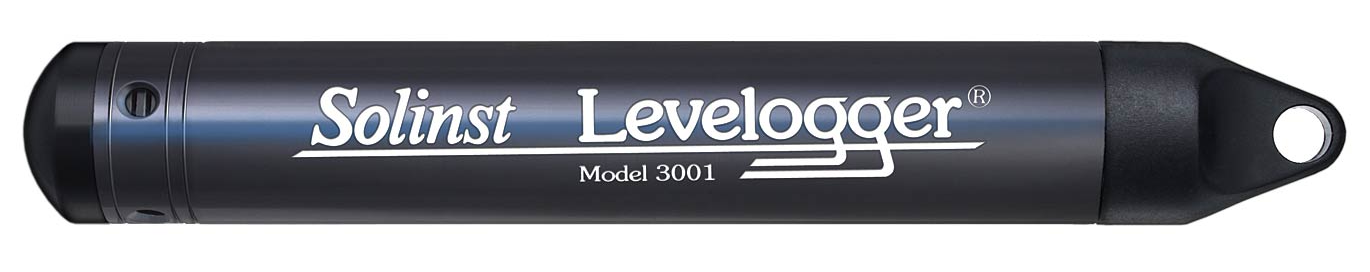
\includegraphics[width=\textwidth]{img/Solinst_EdgeLeveLogger}
                % http://aquaterra.pl/levelogger-edge
                \caption{Solinst Levelogger Edge\textsuperscript{\textregistered}}
                \label{subfig:levelogger_solinst}                
        \end{subfigure}%
        \\[0.5cm]
        \begin{subfigure}[t]{0.5\textwidth}
                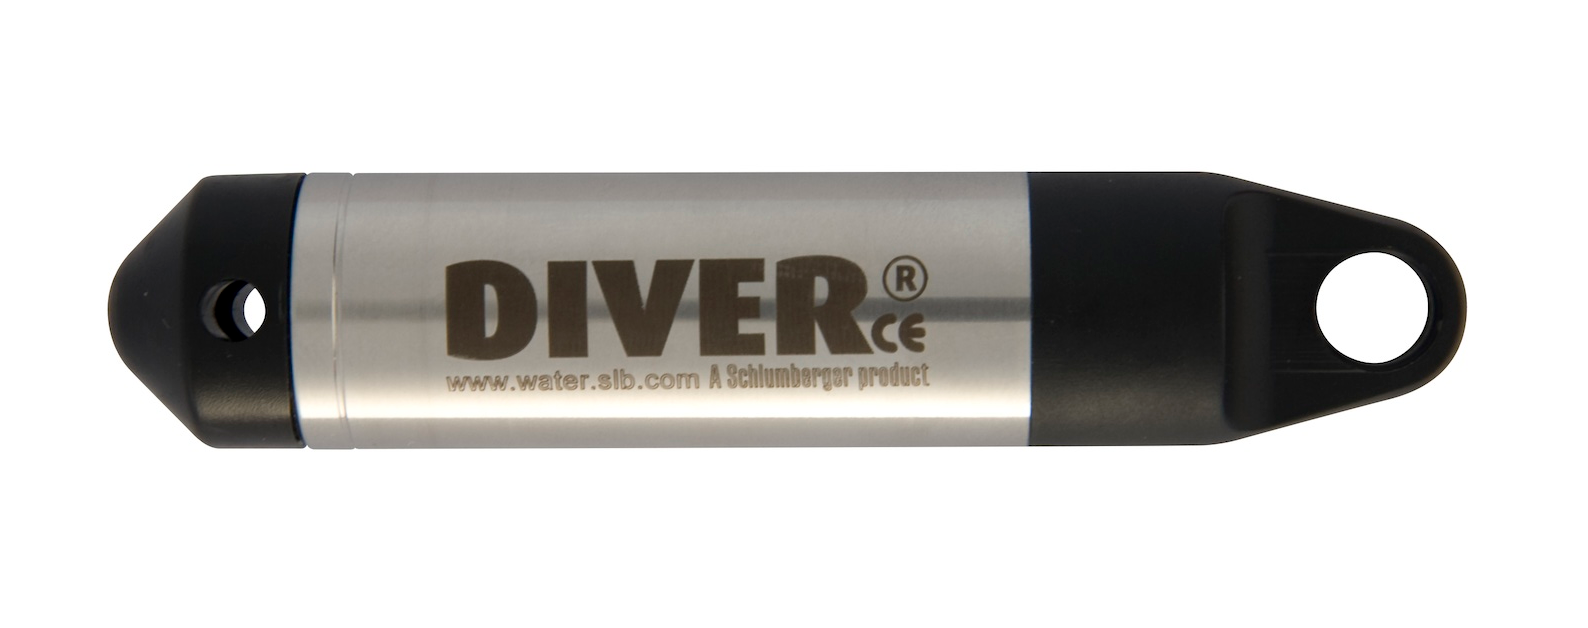
\includegraphics[width=\textwidth]{img/Schlumberger_MiniDiver}
                % http://environnement.sdec-france.com
                \caption{Schlumberger Micro-Diver\textsuperscript{\textregistered}}
                \label{subfig:levelogger_schlumberger}
        \end{subfigure}       
\end{figure}

\cite{freeman_use_2004} provides a guide to the proper selection, installation, and operation of submersible pressure transducers and data loggers for the collection of hydrologic data, primarily for the collection of water-level data from wells.

These instrument are generally suspended at a fixed depth in a well or the piezometer from a stable fixed point called the hanging point, often secured directly to the well casing itself.

These instruments record the absolute pressure (non-vented) and their output must be compensated for barometric pressure in order to obtain a measure of the water level elevation. This is done by subtracting the barometric record from the water-level record. This gives the height of the water column above the instrument.  

Some instrument record the absolute gage pressure. Is measured in reference to atmospheric pressure at mean sea level. Pressures measured by a gage-pressure transducer are positive for pressures greater than sea-level pressure and negative for pressure less than sea-level pressure. Thus, atmospheric pressure measurements above sea-level datum are negative because atmospheric pressure decreases with altitude.

The new

Pressure changes occur in response to changes in the height, and thus in the weight of the water column in the well above the transducer.

DEPTH OF INSTALLATION

The principal objective of selecting a submergence depth at which to hang a transducer during installation is to ensure that water levels do not exceed the transducer’s operational range or fall below it during the monitoring period. Historical water-level measurements can be helpful when designing a long-term water-level monitoring program (Taylor and Alley, 2001). If enough measurements have been made, it is much easier to determine what daily or seasonal extremes can be expected for a given well. Thus, the appropriate range for a transducer can be selected, and its optimum position estimated. To minimize potential for errors and simplify subsequent data processing, reposition the transducer infrequently. Under ideal conditions, the transducer can be hung at a single depth for the entire monitoring period, although it may be necessary to re-position a transducer once

When data have been collected for a sufficient amount of time, WHAT can provides useful insight about past water level comportment and can also be used as a tool for predictive scenario. This can help to better design the optimal depth of installation of the instrument.
 
Even though there exists software that can correct data automatically for barometric pressure, it is still advise to have a basic understanding of the theory.

This is particularly usefull to correct situations when something goes wrong. For example, the barologger may had a deficiency and atmospheric pressure needed to be taken from the CDCD for example and data needed to be corrected manually. There arise often situation when correction needs to be done manually. This happens when there is a problem with the data. This is then good practice to understand the process in order to dodge mistake.

It is a good idea to monitor water level at a 15 min frequency for a period of a year, or more if it is possible. The data can be used subsequently to estimate the barometric response function of the well that can be quite useful to understand the hydrogeological context, and the level of confinement of the well. Having data with this frequency is also useful for running FFT and understand the cause of possible unatural fluctuation in the well.

\begin{figure}[!ht]
\centering
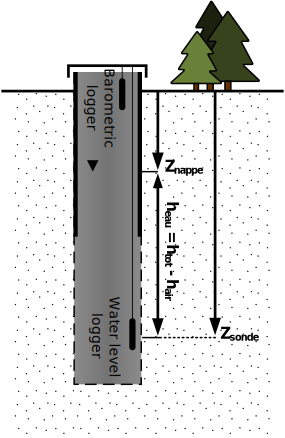
\includegraphics[width=0.5\textwidth]{img/ObsWell}
\caption[Typical instrument configuration for water level monitoring in an observation well]{Typical instrument configuration for water level monitoring in an observation well}
\label{fig:obswell_config}
\end{figure}

Observations of land use, or changes in the general area of the site can be important for data analysis, record compu-tation, and data interpretation. These observations could be notes on land-use changes, construction of new wells nearby, notes of flowmeter readings from production wells, mention of known floods or earthquakes that occurred since the last visit, or any other item that might have a bearing on data collection.


\subsection{Format des données brutes}

Cela implique que pour pouvoir calculer la hauteur de la colonne d'eau, heau, située au-dessus des sondes (voir figure 1), la pression atmosphérique doit également être connue à chacun des puits. À cet effet, des sondes barométriques ont également été installées dans la majorité des puits d'observation du projet Montérégie Est. Une attention particulière a été portée afin d'assurer que les puits qui n'étaient pas munis d'une sonde barométrique étaient situés à proximité et à une altitude raisonnablement similaire d'un puits où la pression atmosphérique était mesurée.

La profondeur de la nappe par rapport à la surface, Znappe, est calculée via l'équation suivante : 

où Znappe (m) et Zsonde (m) correspondent respectivement à la position de la nappe et la profondeur d'installation de la sonde à niveaux d'eau par rapport à la surface du sol, htot (m) est la charge totale mesurée par la sonde à niveaux d'eau et hatm (m) est la charge mesurée par la sonde barométrique. L'axe des z est défini positif vers le haut avec, pour niveau de référence, la surface du sol. Ainsi Zsonde et Znappe ont des valeurs qui sont généralement inférieures à zéro, à moins que le niveau de l'eau dans le puits ne soit situé au-dessus de la surface.

Au cours du projet, trois modèles de sondes ont été utilisés pour la mesure des niveaux d’eau: (1) levelogger Gold de Solinst, (2) levelogger Edge de Solinst et (3) Micro-Diver de Schlumberger. Parallèlement, deux modèles de sondes ont été utilisés pour la mesure de la pression atmosphérique: (1) barologger Gold de Solinst et (2) barologger Edge de Solinst. Il est important de savoir que la méthode de stockage des données brutes varie d'un instrument à l'autre. C’est-à-dire que des transformations mathématiques sont parfois appliquées sur les mesures avant de les mettre en mémoire. En général, cela ne cause pas de problème car les logiciels de traitement des données fournis par les fabricants gèrent le tout de façon automatique et implicite. Par contre, lorsqu'une manipulation manuelle des données brutes est nécessaire ou lorsque des analyses plus complexes sont envisagées, une connaissance des différentes stratégies de stockage des instruments est essentielle.
Pour les sondes levelogger et barologger Gold, les données brutes enregistrées par les instruments correspondent aux pressions mesurées, converties en hauteur d'eau équivalente, moins une constante dont la valeur est établie en fonction de la pression atmosphérique minimale anticipée au niveau de la mer et de l'altitude fournie à la sonde par l'utilisateur lors de sa programmation (9.5 m - 0.0012 m par mètre d'altitude). Pour les sondes Micro-Diver et Levelogger Edge, les données brutes enregistrées par les instruments correspondent aux pressions mesurées converties en hauteur d'eau équivalente. Enfin, pour les sondes barologger Edge, la pression atmosphérique est directement mise en mémoire sans aucune transformation préalable. Le Tableau 1 résume les différentes opérations mathématiques qui sont appliquées aux mesures avant de les mettre en mémoire pour les différents types de sondes qui furent utilisées au cours du projet Montérégie.

où Ptot (kPa) est la pression absolue ressentie par la sonde à niveaux d'eau, Patm (kPa) est la pression atmosphérique, ρ (kg/m3) est la masse volumique de l'eau, g (m/s2) est l'accélération gravitationnelle terrestre et Zalt (m) est l'altitude du puits fourni à la sonde par l'utilisateur lors de sa programmation.

\end{document}